% Slide 3 -- Imaging context
\begin{frame}{Imaging context: why fat-suppressed axial MRI?}
  \begin{columns}[T]
    \begin{column}{0.55\textwidth}
      \begin{block}{Fat saturation (fs)}
        \begin{itemize}
          \item Selective RF pulse \alert{nulls fat signal} $\Rightarrow$ subcutaneous and marrow fat appear dark.
          \item Cortical bone, tendon, edema and joint fluid become \alert{conspicuous}.
          \item Standard sequences here: \textbf{PD-fs} (anatomical detail + edema sensitivity) and \textbf{T1-fs}.
        \end{itemize}
      \end{block}

      \begin{block}{Why the axial plane?}
        \begin{itemize}
          \item The humeral head appears as \alert{nested circles} that grow to a maximum (the ``equator'') and shrink.
          \item Yields a clean \emph{area-vs-slice} curve we can validate geometrically.
          \item Direct view of the glenohumeral contact surface where most tears manifest.
        \end{itemize}
      \end{block}
    \end{column}
    \begin{column}{0.45\textwidth}
      \centering
      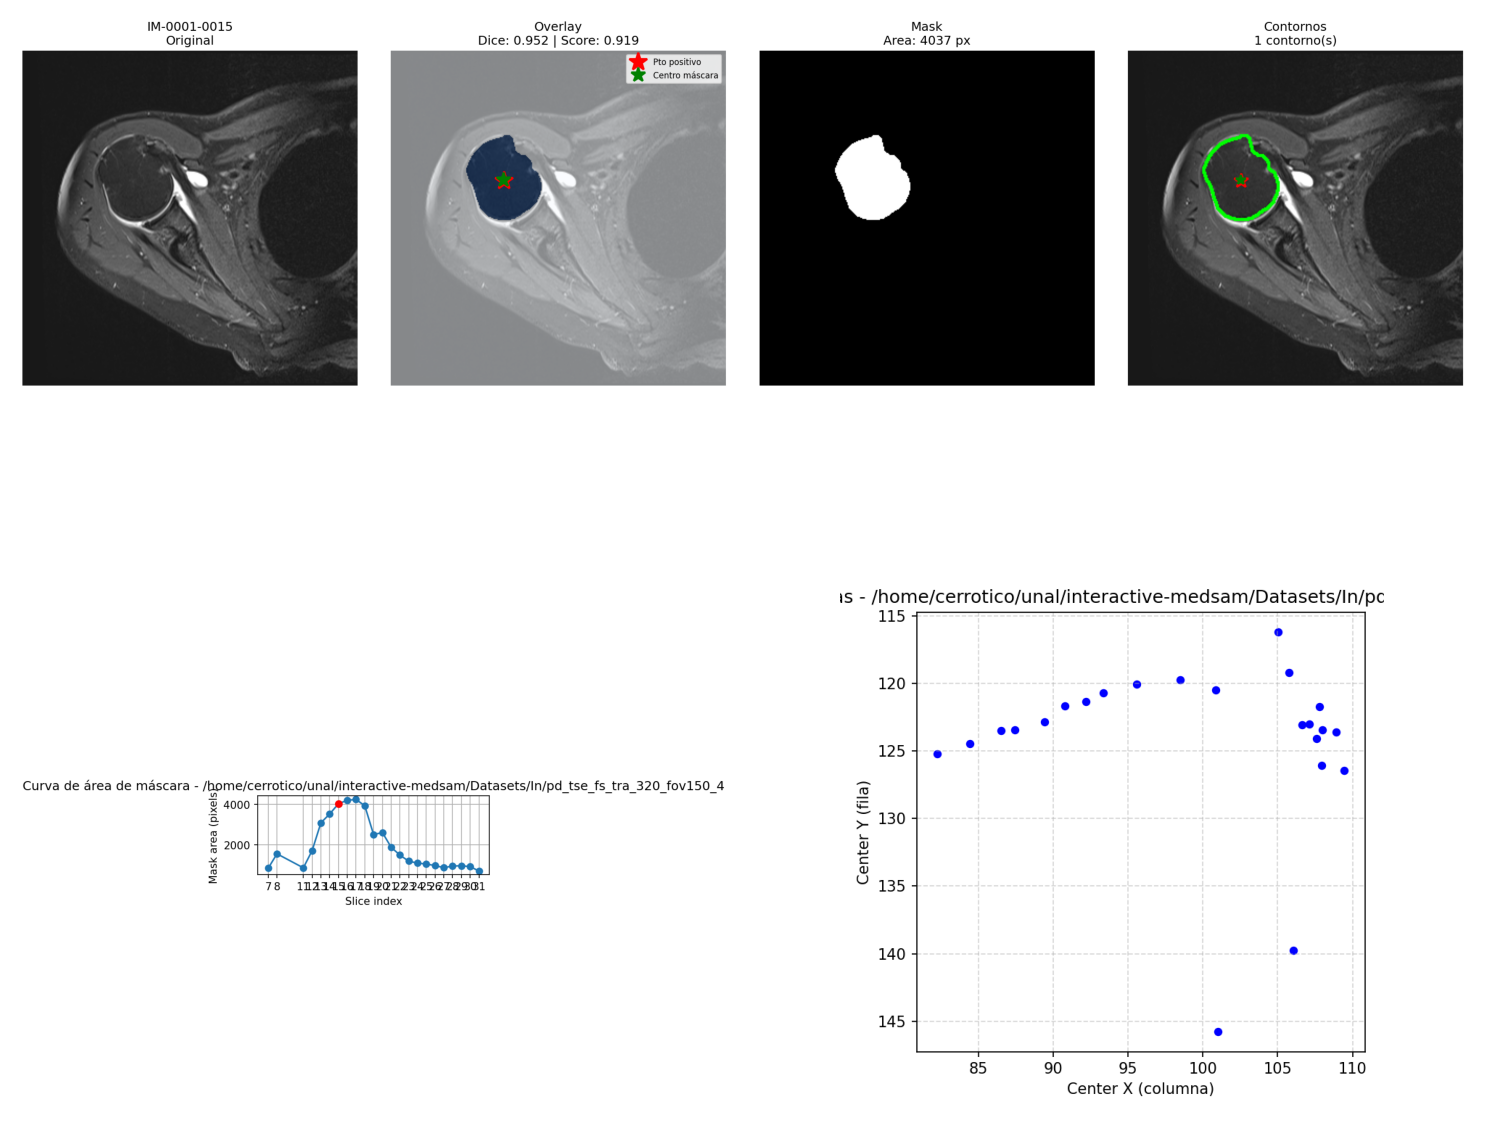
\includegraphics[width=\linewidth]{figures/seg_example.png}
      \\[0.2em]
      {\footnotesize Axial PD-fs slice with humeral segmentation overlay\\ \textit{(PixelSpacing $\approx$ 0.47\,mm; matrix 320$\times$320)}}
    \end{column}
  \end{columns}
\end{frame}
